\section{Mean-Reversion Diagnostic} \label{ap:regmedia}

This appendix compares the main specification with the baseline-support restriction. The goal is to assess whether the main results depend on comparing initially low-performing treated schools with controls far away in the pre-treatment distribution.

\subsection{Event Studies by Model}

\begin{figure}[!htbp]
    \centering
    \caption{Mean-reversion diagnostic: 9th grade, Portuguese Language}
    \label{fig:ap_regmedia_9ef_lp}
    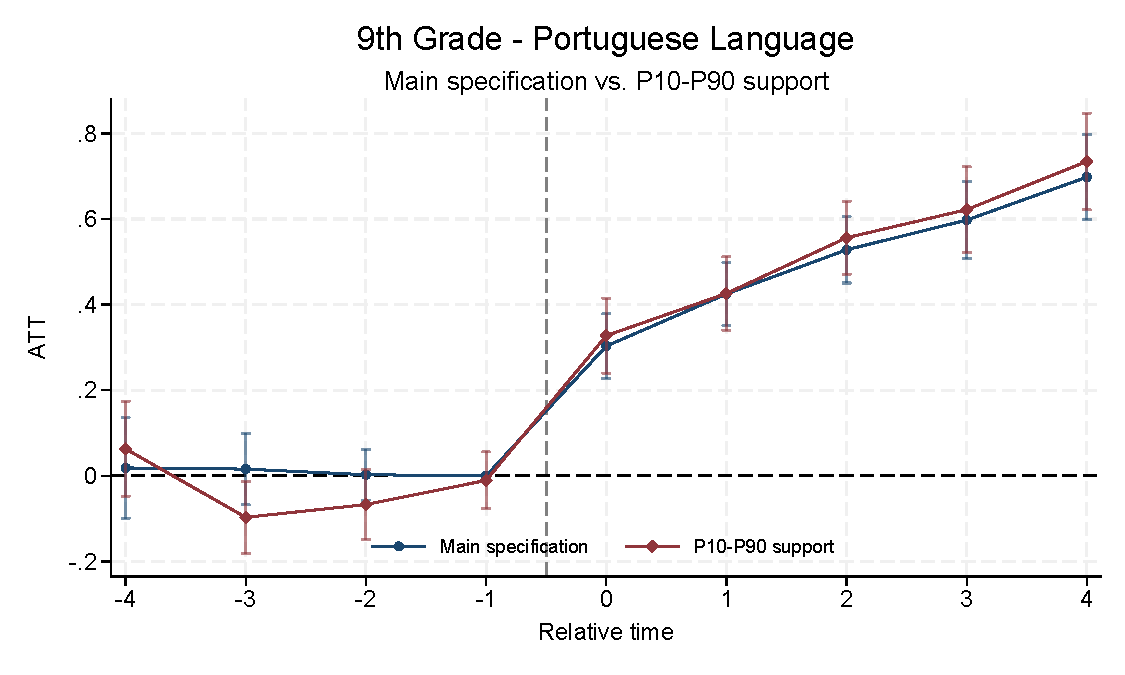
\includegraphics[width=0.88\textwidth]{files/images/appendix/eventstudy_regmedia_9EF_LP.pdf}
    \\ \vspace{0.1cm}
    \footnotesize{Source: author's elaboration. The restricted line uses schools within the P10--P90 support of baseline proficiency among treated schools.}
\end{figure}

\begin{figure}[!htbp]
    \centering
    \caption{Mean-reversion diagnostic: 9th grade, Mathematics}
    \label{fig:ap_regmedia_9ef_mat}
    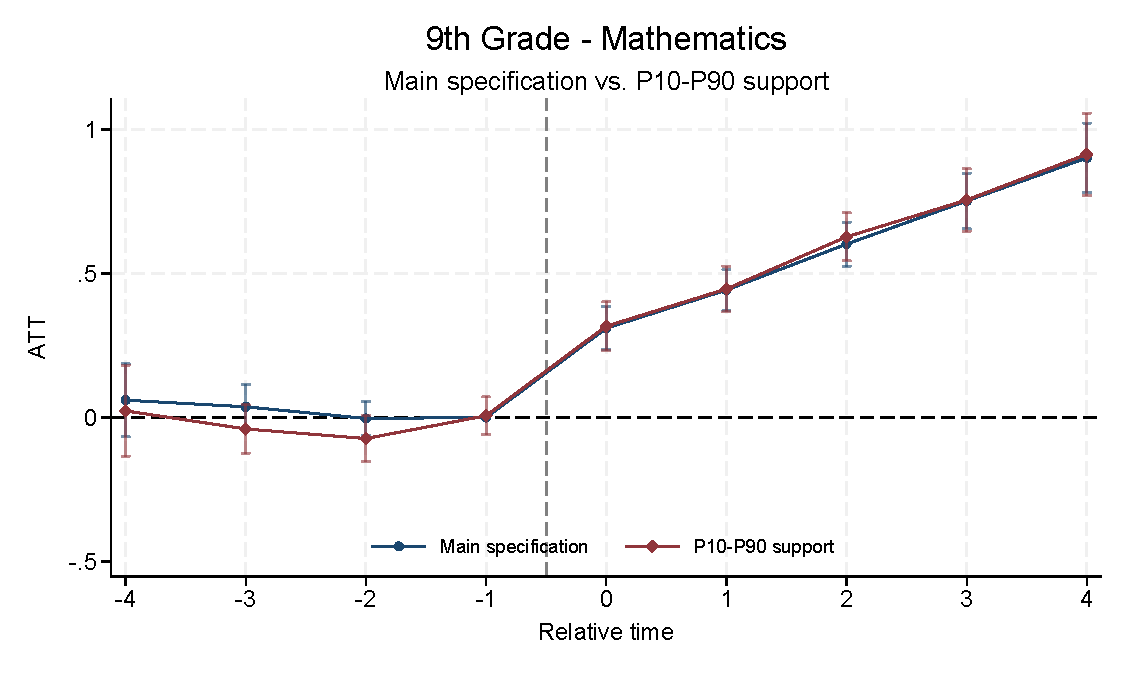
\includegraphics[width=0.88\textwidth]{files/images/appendix/eventstudy_regmedia_9EF_Mat.pdf}
    \\ \vspace{0.1cm}
    \footnotesize{Source: author's elaboration. The restricted line uses schools within the P10--P90 support of baseline proficiency among treated schools.}
\end{figure}

\begin{figure}[!htbp]
    \centering
    \caption{Mean-reversion diagnostic: 3rd grade of high school, Portuguese Language}
    \label{fig:ap_regmedia_em3_lp}
    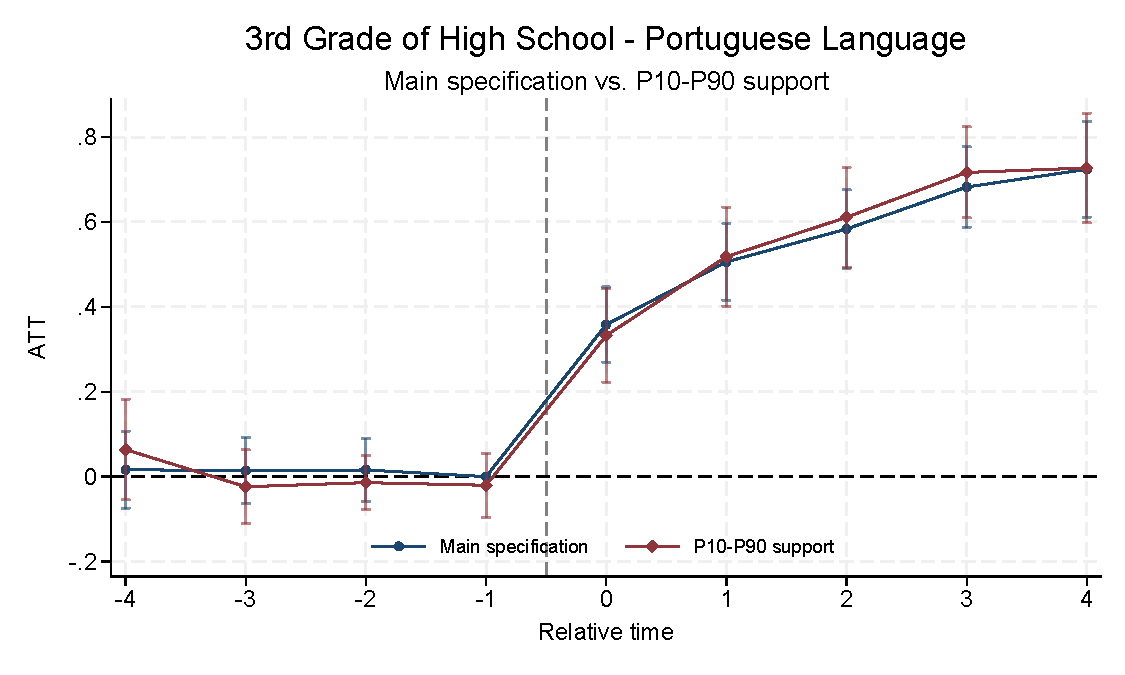
\includegraphics[width=0.88\textwidth]{files/images/appendix/eventstudy_regmedia_EM3_LP.pdf}
    \\ \vspace{0.1cm}
    \footnotesize{Source: author's elaboration. The restricted line uses schools within the P10--P90 support of baseline proficiency among treated schools.}
\end{figure}

\begin{figure}[!htbp]
    \centering
    \caption{Mean-reversion diagnostic: 3rd grade of high school, Mathematics}
    \label{fig:ap_regmedia_em3_mat}
    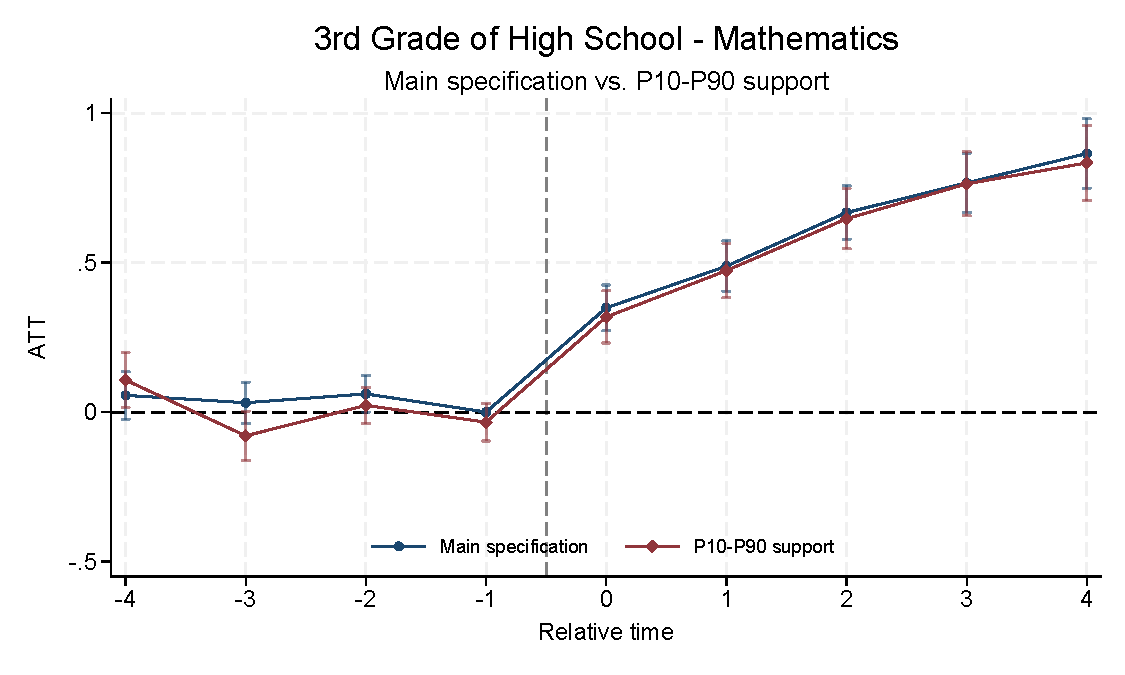
\includegraphics[width=0.88\textwidth]{files/images/appendix/eventstudy_regmedia_EM3_Mat.pdf}
    \\ \vspace{0.1cm}
    \footnotesize{Source: author's elaboration. The restricted line uses schools within the P10--P90 support of baseline proficiency among treated schools.}
\end{figure}

\subsection{ATT by Period}

\begin{table}[!htbp]
\centering
\caption{Mean-reversion diagnostic, 9th LP: ATT by relative period}
\label{tab:ap_event_regmedia_9th_lp}
\vspace{-0.15cm}
\scriptsize
\setlength{\tabcolsep}{4pt}
\renewcommand{\arraystretch}{0.92}
\begin{tabular}{lcc}
\toprule
Relative period & Main & P10-P90 support \\
\midrule
-4 & 0.019 (0.060) & 0.063 (0.057) \\
-3 & 0.016 (0.043) & -0.097 (0.043) \\
-2 & 0.003 (0.030) & -0.067 (0.042) \\
-1 & 0.000 & -0.011 (0.034) \\
0 & 0.303 (0.039) & 0.327 (0.045) \\
1 & 0.425 (0.038) & 0.426 (0.044) \\
2 & 0.528 (0.040) & 0.556 (0.044) \\
3 & 0.598 (0.046) & 0.622 (0.051) \\
4 & 0.698 (0.051) & 0.734 (0.058) \\
\bottomrule
\end{tabular}
\begin{flushleft}
\footnotesize Note: each cell reports the ATT and standard error in parentheses, in standard deviations of annual proficiency. Period \(k=-1\) is normalized as the baseline and therefore appears without a standard error.
\end{flushleft}
\end{table}




\begin{table}[!htbp]
\centering
\caption{Mean-reversion diagnostic, 9th Math: ATT by relative period}
\label{tab:ap_event_regmedia_9th_mat}
\vspace{-0.15cm}
\scriptsize
\setlength{\tabcolsep}{4pt}
\renewcommand{\arraystretch}{0.92}
\begin{tabular}{lcc}
\toprule
Relative period & Main & P10-P90 support \\
\midrule
-4 & 0.060 (0.065) & 0.023 (0.081) \\
-3 & 0.037 (0.040) & -0.040 (0.043) \\
-2 & -0.003 (0.030) & -0.073 (0.041) \\
-1 & 0.000 & 0.006 (0.033) \\
0 & 0.310 (0.038) & 0.317 (0.043) \\
1 & 0.442 (0.036) & 0.446 (0.040) \\
2 & 0.602 (0.039) & 0.627 (0.043) \\
3 & 0.751 (0.049) & 0.755 (0.055) \\
4 & 0.901 (0.062) & 0.914 (0.073) \\
\bottomrule
\end{tabular}
\begin{flushleft}
\footnotesize Note: each cell reports the ATT and standard error in parentheses, in standard deviations of annual proficiency. Period \(k=-1\) is normalized as the baseline and therefore appears without a standard error.
\end{flushleft}
\end{table}




\begin{table}[!htbp]
\centering
\caption{Mean-reversion diagnostic, HS3 LP: ATT by relative period}
\label{tab:ap_event_regmedia_HS3_lp}
\vspace{-0.15cm}
\scriptsize
\setlength{\tabcolsep}{4pt}
\renewcommand{\arraystretch}{0.92}
\begin{tabular}{lcc}
\toprule
Relative period & Main & P10-P90 support \\
\midrule
-4 & 0.016 (0.046) & 0.064 (0.060) \\
-3 & 0.014 (0.040) & -0.024 (0.044) \\
-2 & 0.016 (0.038) & -0.014 (0.032) \\
-1 & 0.000 & -0.020 (0.038) \\
0 & 0.358 (0.045) & 0.333 (0.056) \\
1 & 0.506 (0.046) & 0.518 (0.059) \\
2 & 0.583 (0.047) & 0.611 (0.060) \\
3 & 0.682 (0.048) & 0.717 (0.055) \\
4 & 0.724 (0.058) & 0.727 (0.066) \\
\bottomrule
\end{tabular}
\begin{flushleft}
\footnotesize Note: each cell reports the ATT and standard error in parentheses, in standard deviations of annual proficiency. Period \(k=-1\) is normalized as the baseline and therefore appears without a standard error.
\end{flushleft}
\end{table}




\begin{table}[!htbp]
\centering
\caption{Mean-reversion diagnostic, HS3 Math: ATT by relative period}
\label{tab:ap_event_regmedia_HS3_mat}
\vspace{-0.15cm}
\scriptsize
\setlength{\tabcolsep}{4pt}
\renewcommand{\arraystretch}{0.92}
\begin{tabular}{lcc}
\toprule
Relative period & Main & P10-P90 support \\
\midrule
-4 & 0.056 (0.041) & 0.107 (0.047) \\
-3 & 0.031 (0.035) & -0.080 (0.042) \\
-2 & 0.061 (0.031) & 0.022 (0.031) \\
-1 & 0.000 & -0.034 (0.032) \\
0 & 0.349 (0.039) & 0.318 (0.044) \\
1 & 0.488 (0.043) & 0.473 (0.046) \\
2 & 0.667 (0.045) & 0.647 (0.051) \\
3 & 0.767 (0.051) & 0.763 (0.054) \\
4 & 0.865 (0.059) & 0.834 (0.064) \\
\bottomrule
\end{tabular}
\begin{flushleft}
\footnotesize Note: each cell reports the ATT and standard error in parentheses, in standard deviations of annual proficiency. Period \(k=-1\) is normalized as the baseline and therefore appears without a standard error.
\end{flushleft}
\end{table}





